\subsection{Fisión y fusión nuclear}
    
Las reacciones nucleares —aquellas en las que participan los núcleos atómicos— pueden tener lugar espontáneamente, como en la radiactividad, o pueden ser inducidas por el bombardeo con una partícula o un haz. Las reacciones nucleares son mucho más
energéticas que las reacciones químicas, pero obedecen a las mismas leyes físicas: conservación de la cantidad de movimiento,
energía, número de partículas y carga. En la actualidad la cantidad de posibles reacciones nucleares es enorme, ya que existen aproximadamente 2000 isótopos conocidos y una gran cantidad de partículas que pueden ser utilizadas como proyectiles.  \cite{Murray.2020}\\
En una reacción nuclear, dos núcleos, o un nucleón, y un núcleo, se aproximan tanto que interactúan mediante la interacción fuerte. \cite{Cottingham.2001}\\ 
Una reacción nuclear se puede definir como una colisión entre dos núcleos que produce un
cambio en la composición nuclear y/o en el estado de energía de la interacción
núcleo. En circunstancias normales, las reacciones nucleares ocurren cuando un objetivo es bombardeado por partículas/núcleos provenientes de un acelerador o de una sustancia radiactiva.\\
Cuando dos núcleos o un núcleo y una partícula colisionan, Pueden ocurrir los siguientes escenarios: 
\begin{enumerate}
    \item \textbf{Dispersión} se da cuando el proyectil incidente se encuentra entre los resultados de la reacción. La dispersión puede ser:
    \begin{itemize}
        \item \textit{Elástica}: Se da cuando los núcleos que interactúan permanecen sin cambio y no se crean nuevas partículas. Solo existe una redistribución de las energías cinéticas de las partículas. Ejemplo:
        \begin{equation*}
            p+^{16}O \longrightarrow p+^{16}O
        \end{equation*}
        En este caso tanto el núcleo como el proyectil permanecen sin cambio, únicamente pueden cambiar la velocidad o la dirección de los elementos interactuantes. 
    \item \textit{Inelástica}: Se da cuando el núcleo o el proyectil se excitan después de la colisión, se fracturan formando nuevas partículas. En este tipo de reacciones parte de la energía cinética del sistema se convierte en energía interna. Ejemplo:
    \begin{equation*}
         n+^{16}O \longrightarrow n+^{16}O^*
    \end{equation*}
    El oxígeno termina en un estado excitado. 
    \end{itemize}
 \item \textbf{Transmutación} ocurre cuando se da un reordenamiento de los constituyentes nucleares dentro de los núcleos interactuantes. Ejemplo:
 \begin{equation*}
         d+^{14}N \longrightarrow ^{3}He+^{13}C
    \end{equation*}
\end{enumerate}
En esta reacción podemos observar como el núcleo de nitrógeno pierde un protón, convirtiéndose así en un núcleo de carbón. Mientras el núcleo de deuterio (d) adquiere este protón y se convierte en un núcleo de helio. 
Estas reacciones también pueden resultar en más de dos núcleos finales. Por ejemplo:
 \begin{equation*}
         \gamma+^{233}U \longrightarrow ^{90}Rb+^{141}Cs+2n
    \end{equation*}
Podemos observar en esta reacción que el núcleo de uranio se dividió en 2 núcleos más, más dos neutrones. \cite{Sanctis.2016}\\

Clasificaremos las reacciones nucleares existentes en dos grupos principales: reacciones de fisión y reacciones de fusión.



\subsubsection{Reacciones de Fisión}
La fisión es la ruptura espontánea o inducida de un núcleo. Si bien es “simplemente otra reacción” desde el punto de vista de la física, tiene un papel especial en asuntos públicos debido a sus enormes aplicaciones en la producción de energía y armamentos. \cite{Basdevant.2005}\\

En la fisión nuclear, el núcleo de un elemento pesado se divide en unos pocos
fragmentos más ligeros (generalmente dos, la llamada fisión binaria), liberando una gran cantidad de energía y un cierto número de neutrones libres (típicamente dos o tres). \cite{Murray.2020}
\begin{figure}[H]
    \centering
    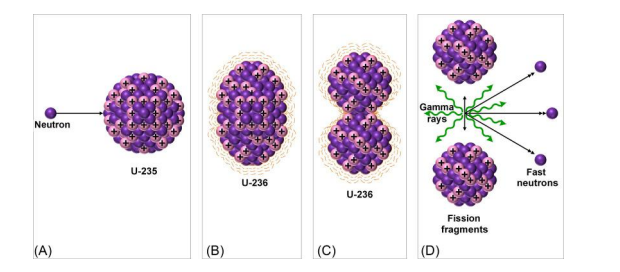
\includegraphics[scale=.55]{imagenes/fision nuclear.png}
    \caption{Proceso de fisión inducido, un neutrón interactúa con un núcleo de U-235, formando U-236, que luego se fisiona en dos partes, liberando energía y neutrones.\cite{Murray.2020}}
    \label{fig:fision}
\end{figure}
En comparación con reacciones químicas como la combustión de combustibles fósiles, la fisión requiere un volumen mucho menor de material combustible para producir una equivalente cantidad de energía. Para hacer la comparación más cuantitativa, la energía liberada por fisión de 1 gramo de U-235 es de unos 82 mil millones julios, equivalente a la liberada al quemar alrededor de tres millones gramos de carbón. \cite{Sanctis.2016}

\subsubsection{Reacciones de Fusión}
La fusión nuclear es la combinación de dos o más núcleos en un núcleo más pesado. Durante este proceso la suma de las masas de los constituyentes individuales es mayor que la masa del nuevo núcleo formado. Supongamos que se pueden combinar dos núcleos de hidrógeno y dos neutrones para
formar el núcleo de helio. En la reacción:
\begin{equation*}
    2^1_1H+2^1_0n \longrightarrow^4_2 He
\end{equation*}
El defecto de masa energía está dado por:
\begin{align}
    \nonumber \Delta m&=\Sigma M_{react}- M_{prod}\\
    \nonumber &=2M_{H-1}+2m_n-M_{He-4}\\
    \nonumber 0.030377&=2(1.007825)+2(1.008665)\\
    \nonumber &-4.002603\left[amu\right]
\end{align}
Lo que corresponde a 28.3 MeV de energía. \cite{Murray.2020}

Las reacciones de fusión, que tienen lugar en el Sol, siempre han sido la fuente principal de energía en la Tierra. En la Tierra, la vez que el humano manipuló esta energía fue en 1952, durante las pruebas de la bomba de hidrógeno. Desde entonces la humanidad ha tenido la ambición de domar esta forma de energía. Es más limpia que la fisión, creando muchos menos desechos radiactivos de vida larga. Sus recursos son ilimitados. En 300 litros de agua de mar hay 1 gramo de deuterio. El agua en los océanos podría proporcionar suficiente energía para las necesidades humanas durante varios cientos de millones de años. Es particularmente frustrante ver que, a diferencia de la fisión que se utilizó industrialmente unos años después de su descubrimiento, la fusión aún se encuentra en una etapa prospectiva más de 50 años después de su primer uso terrestre. \cite{Basdevant.2005}

Hasta ahora, un dispositivo práctico de energía de fusión no ha sido demostrado, y considerable investigación y desarrollo será necesario para alcanzar ese objetivo. \cite{Murray.2020}

\begin{figure}[H]
    \centering
    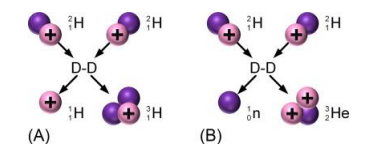
\includegraphics[scale=.65]{imagenes/fusion nuclear.png}
    \caption{Ejemplos de reacciones de fusión deuterio-deuterio (A) deuterio-deuterio (p) (B) deuterio-deuterio (n).\cite{Murray.2020}}
    \label{fig:fision}
\end{figure}
\subsection{Energía de desintegración}
Una reacción nuclear típica la podemos escribir como:
\begin{equation*}
  a + X \longrightarrow Y + b  
\end{equation*}
Aplicando conservación de la energía relativista podemos escribir la reacción como:
\begin{equation}
    m_Xc^2+T_x+m_ac^2+T_a\ \longrightarrow m_Yc^2+T_Y+m_bc^2+T_b
\end{equation}

Donde T representa la energía cinética de las partículas, en el ámbito no relativista podemos utilizar ($T=\frac{1}{2}mv^2$). Las m´s representan las masas en reposo de las partículas. Definiremos el valor Q (energía de la reacción o energía de desintegración) como:
\begin{equation}
    Q=(m_{inicial}-m_{final})c^2   
\end{equation}
También se puede expresar como el exceso de la energía final de los productos.
\begin{equation}
   Q=T_{final}-T_{inicial}
\end{equation} 
\begin{equation}
   Q=T_Y+T_b-T_X-T_a
\end{equation}
El valor de Q puede ser positivo o negativo. Si Q es negativo o cero, entonces se dice que la reacción es exotérmica. En este caso la masa nuclear o la energía de enlace se libera como energía cinética de los productos finales. Si el valor de Q es positivo, entonces la se dice que la reacción es endotérmica. En este caso la energía cinética inicial es convertida en masa nuclear o en energía de enlace. \cite{Krane.1987}
\subsection{Materiales fisionables}
La fisión de un núcleo en particular puede producir una gran cantidad de diferentes fragmentos. Por ejemplo para la captura neutrónica de un átomo de $^{235}U_{92}$ para formar $^{236}U_{92}$  podemos tener: \cite{Sanctis.2016}
\begin{figure}[H]
    \centering
    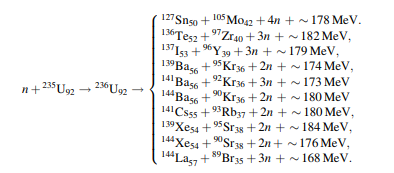
\includegraphics[scale=.925]{imagenes/posibilidades.png}
    \caption{Posibles resultados que se pueden obtener de la captura neutronica de $^{235}U_{92}$ para formar $^{236}U_{92}$.\cite{Sanctis.2016}}
    \label{fig:posibilidades}
\end{figure}        
Los núcleos pesados los cuales son estables o casi estables tienen una relación alta entre protones y neutrones a diferencia de los núcleos ligeros que tienden a tener aproximadamente la misma cantidad de neutrones y protones. Esta diferencia implica que al fisionarse los productos también serán ricos en neutrones. Por lo general lo productos de la fisión son inestables, poseyendo demasiados neutrones para un núcleo de su  numero másico, eventualmente decaerán mediante $\beta^-$ hasta formar un núcleo mas estable. 
\subsection{Tipos de centrales nucleares}